\documentclass[15pt]{standalone}
\usepackage{xcolor}
\usepackage{tikz}
\usepackage{pgfplots}
\definecolor{slide}{HTML}{d5002d}
\definecolor{original}{HTML}{005aff}
\definecolor{scaled}{HTML}{03af7a}
\begin{document}
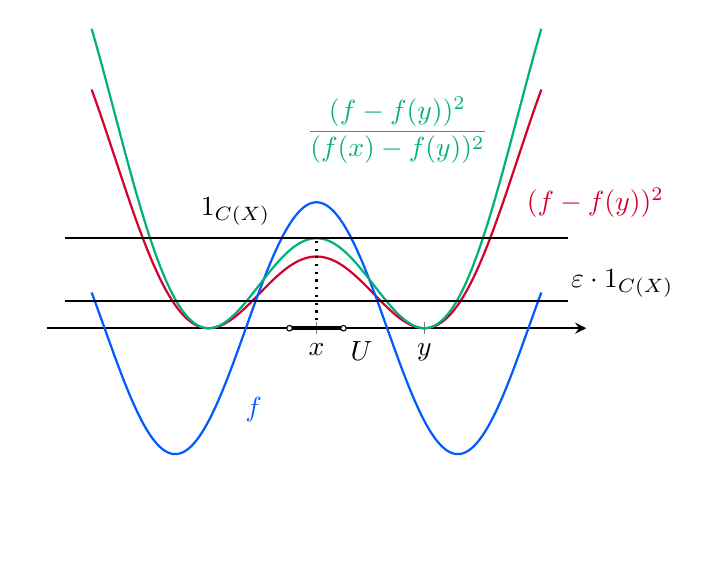
\begin{tikzpicture}
    \begin{axis}[
        axis equal,
        axis x line=middle,
        axis line style=thick,
        xmin=-3,
        xmax=3,
        ymin=-1.8,
        ymax=1.8,
        xtick={0, 1.2},
        xticklabels={$x$, $y$},
        x tick style={draw},
        x axis line style={draw},
        ytick={},
        yticklabels={},
        y axis line style={draw=none},
        y tick style={draw=none},
        samples=300,
        clip=false
    ]
    \def\SCALE{1.4};
    \def\SIGMA{0.3};
    \def\A{-2.5};
    \def\B{2.5};
    \def\b{-0.5};
    \addplot[color=slide, thick][domain=\B:\A] {(- \SCALE * cos(deg(1.2)) + \SCALE * cos(deg(x)))^2};
    \addplot[color=original, thick][domain=\B:\A] {\SCALE * cos(deg(2 * x))};
    \addplot[color=scaled, thick][domain=\B:\A] {(- \SCALE * cos(deg(1.2)) + \SCALE * cos(deg(x)))^2 / (-\SCALE * cos(deg(1.2)) + \SCALE)^2 };
    \node[color=slide] (slide) at (axis cs:3.1, 1.4) {$(f - f(y))^2$};
    \node[color=original] (original) at (axis cs:-0.7, -0.9) {$f$};
    \node[color=scaled] (scaled) at (axis cs:0.9, 2.2) {$\displaystyle \frac{(f - f(y))^2}{(f(x) - f(y))^2}$};

    \draw[fill=white, opacity=1] (axis cs:-0.3, 0) circle[radius=1pt];
    \draw[fill=white, opacity=1] (axis cs:0.3, 0) circle[radius=1pt] {};
    \draw[ultra thick] (axis cs: -0.275, 0) -- (axis cs: 0.275, 0);
    \node[] at (axis cs: 0.5, -0.25) {$U$};

    \draw[thick] (axis cs:-2.8, 1) -- (axis cs:2.8, 1);
    \draw[thick, dotted] (axis cs: 0, 0) -- (axis cs: 0, 1);
    \node[] (line1) at (axis cs:-0.9, 1.3) {$1_{C(X)}$};
    \node[] (line2) at (axis cs:3.4, 0.5) {$\varepsilon \cdot 1_{C(X)}$};
    \draw[thick] (axis cs:-2.8, 0.3) -- (axis cs:2.8, 0.3);

    \end{axis}
    \end{tikzpicture}
\end{document}
